\section{Detecting weather a vessel is fishing at a given point}
One of our primary objectives is to identify vessels that are fishing in maritime protected areas.

International Union for Conservation of Nature - IUCN has defined MPAs as follows:
'A clearly defined geographical space, recognised, dedicated and managed, through legal or other effective means, to achieve the long-term conservation of nature with associated ecosystem services and cultural values'.

MPAs are classified into several categories based on the fishing restrictions. Restrictions may vary from protecting particular species to no fishing allowed.

Being able to identify weather a vessel is fishing at any point along its trajectory will help us identify vessels fishing in MPAs and Exclusive Economic Zones.

\section{Data}

We are using the AIS data provided by \href{https://spire.com/}{Spire}.
AIS transceivers send positional data every 2-10 seconds and static data every 6 minutes.

The positional AIS data contains the following fields:
\begin{itemize}
\item The vessel's Maritime Mobile Service Identity (MMSI) : a unique nine digit identification number.
\item Navigation status : "at anchor", "under way using engine(s)", "not under command", etc.
\item Rate of turn : right or left, from 0 to 720 degrees per minute
\item Speed over ground : 0.1-knot (0.19 km/h) resolution from 0 to 102 knots (189 km/h)
\item Positional accuracy:
Longitude : to 0.0001 minutes
Latitude : to 0.0001 minutes
\item Course over ground : relative to true north to 0.1°
\item True heading : 0 to 359 degrees (for example from a gyro compass)
\item True bearing at own position. 0 to 359 degrees
UTC Seconds : The seconds field of the UTC time when these data were generated.
\end{itemize}

The static data contains the following fields:

\begin{itemize}
\item IMO ship identification number : a seven digit number that remains unchanged upon transfer of the ship's registration to another country
\item Radio call sign : international radio call sign, up to seven characters, assigned to the vessel by its country of registry
\item Name : 20 characters to represent the name of the vessel
\item Type of ship/cargo
\item Dimensions of ship : to nearest meter
\item Location of positioning system's (e.g., GPS) antenna on board the vessel : in meters aft of bow and meters port or starboard
\item Type of positioning system : such as GPS, DGPS or LORAN-C.
\item Draught of ship : 0.1 meter to 25.5 meters
\item Destination : max. 20 characters
\item ETA (estimated time of arrival) at destination : UTC month/date hour:minute
\end{itemize}

We have access to an year of worldwide AIS messages. We also used the training data provided by \href{globalfishingwatch.github.io}{Global Fishing Watch}. The data contains positional data and the labels for weather the vessel was fishing at that point or not. This data set was labeled for 90 vessels over a period of 3 years.

\begin{figure}[H]
\centering
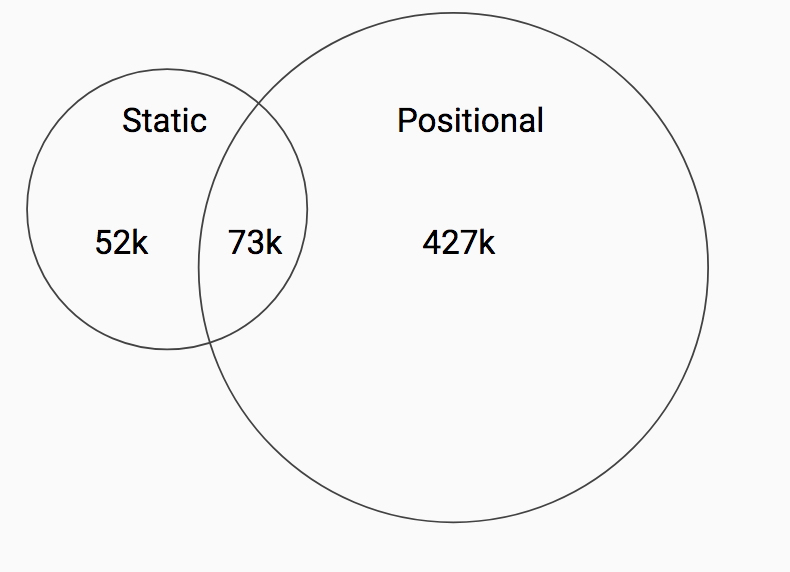
\includegraphics[width=0.5\textwidth]{images/ais_summary.png}
\caption{\label{fig:AIS broadcast summary}Number of positional and static AIS messages for a period of 1 year}
\end{figure}

\section{Modelling}

Here we describe an approach to use AIS data to identify at what points along their trajectory the vessels were fishing.

\subsection{Feature generation}

After discussions with domain experts, we came up with a list of features that might be good indicators of fishing behavior.
We generated features like distance from shore, port, day or night during the time of navigation etc. We then fit a Random Forest model to compute how each of the feature contributes towards the prediction.

\begin{figure}[H]
\centering
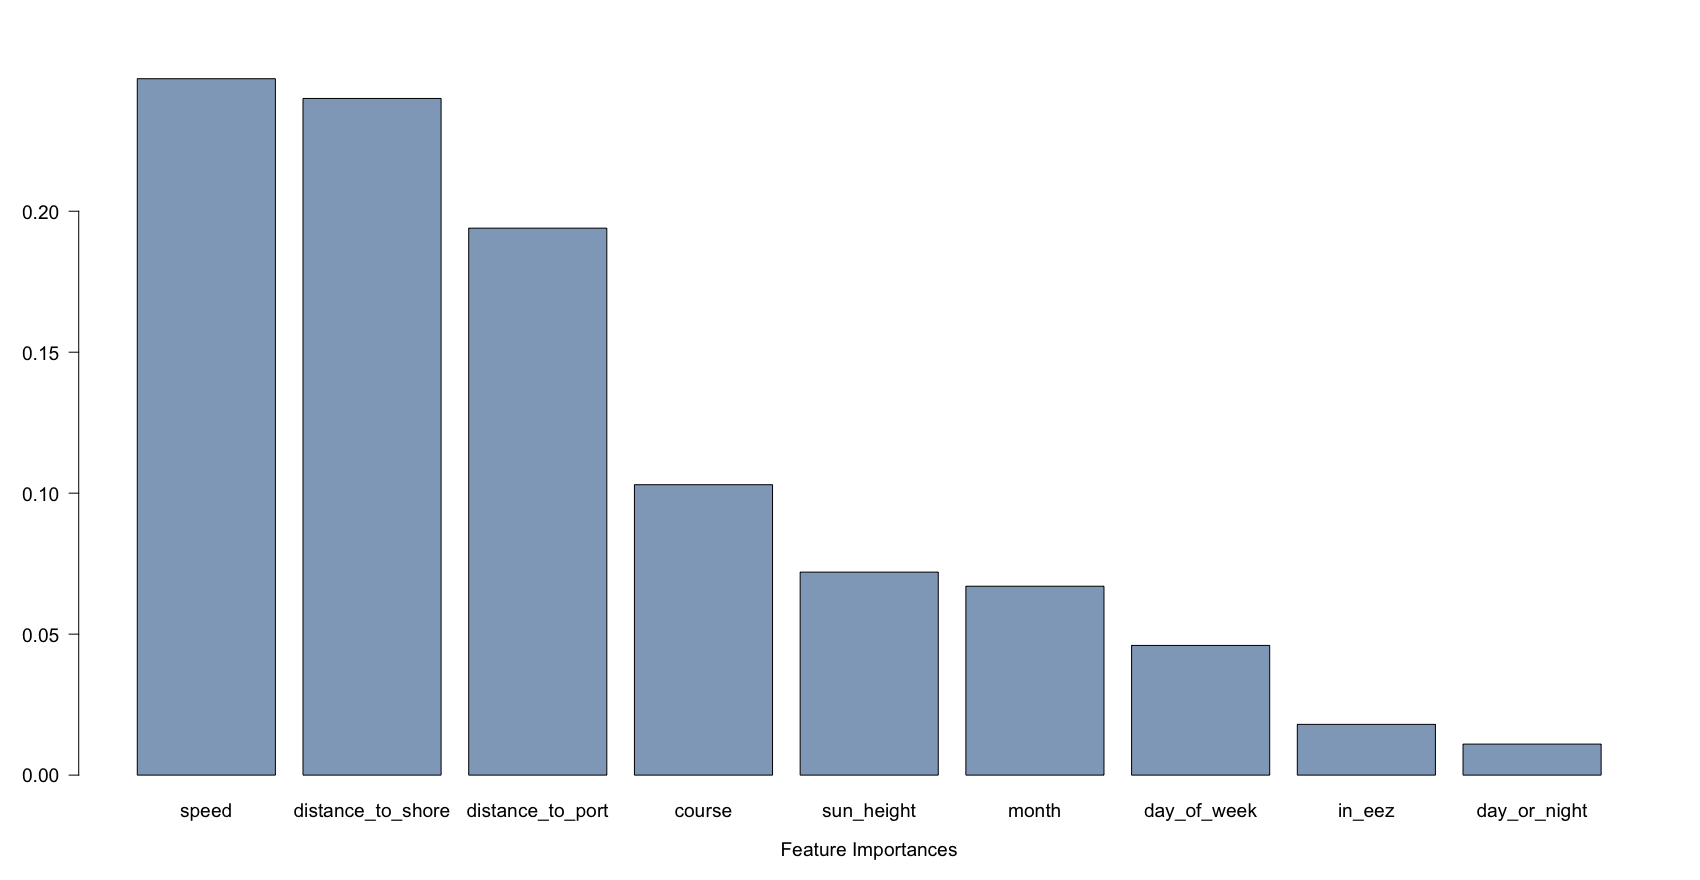
\includegraphics[width=0.5\textwidth]{images/feature_importance_final.png}
\caption{\label{fig:Feature importance}Feature importance for AIS positional features.}
\end{figure}

\subsection{Training and cross-validation}

Given we have a time series data, we split our data set into multiple temporal folds. For each fold, we split the train-test set as illustrated in the following figure.

\begin{figure}[H]
\centering
\includegraphics[width=0.5\textwidth]{images/temporal_cv.png}
\caption{\label{fig:Temporal Cross-validation}Temporal splits for each fold}
\end{figure}

We compute various metrics like precision, recall, false positive and true positives rates etc.

\subsection{Model selection}
After talking to our partners, we came to the conclusion that we want to optimize for precision of our models.
For example, in the following figure, you can see three precision-recall curves. For the model represented by the blue curve, you see high precision at first and then the precision get worse than the same for other models. The models we select also depend on how many cases our partner can act upon. If the partner can act upon K cases, then we should select the model that maximizes precision for those K cases.

\begin{figure}[H]
\centering
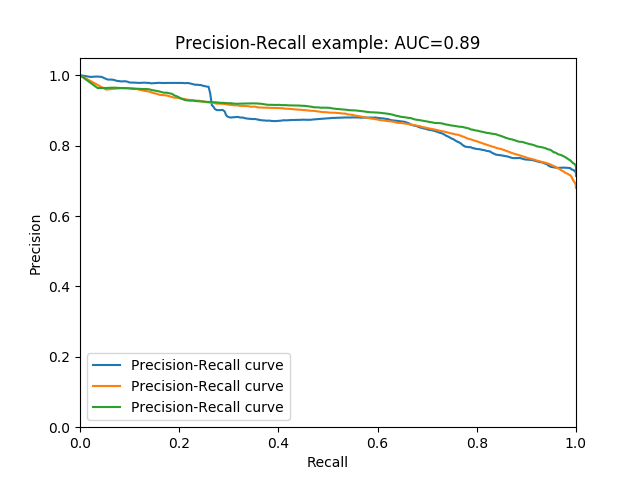
\includegraphics[width=0.5\textwidth]{images/precision_recall_curve.png}
\caption{\label{fig:Precision-Recall}Precision-Recall curve for different models}
\end{figure}

\section{Evaluation}

In the absence of a labeled prediction set, we are employing a few heuristics to examine the performance of our models.
For example, average fishing score for reported fishing vessels should in general, be greater than the same for vessels that don't report themselves as fishing.

	
Vessels spend most of their time being docked. Also, reported fishing vessels spend only a small fraction of their time actually fishing.

\begin{figure}[H]
\centering
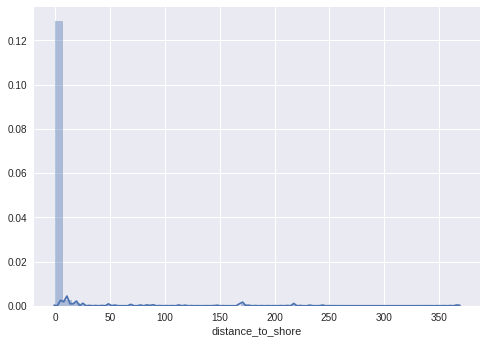
\includegraphics[width=0.5\textwidth]{images/distance_to_shore.png}
\caption{\label{fig:Distance to shore distribution}Distribution of distance to shore in the AIS messages}
\end{figure}


\begin{figure}[H]
\centering
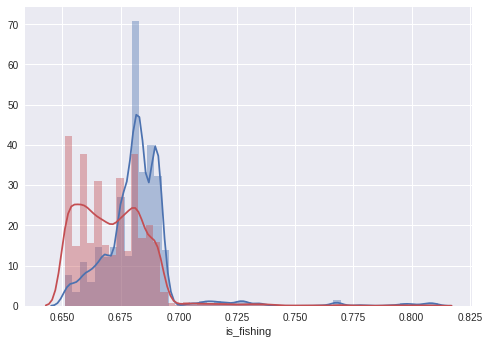
\includegraphics[width=0.5\textwidth]{images/fishing_score_distributions.png}
\caption{\label{fig:Fishing score distribution}Fishing score distributions for reported and non reported fishing vessels.}
\end{figure}
